\subsection{Configuration Editor}
\writer{Albert}

The Configuration Editor is a component that will work as a connector between the Petri net editor (Section \ref{sec:sf-petrinet}), the Geometry editor (Section \ref{sec:sf-geometry}) and the Appearance editor (Section \ref{sec:sf-appearance}). 

\subsubsection{Functional Requirements}

\begin{enumerate}
	\item The Configuration Editor \textbf{shall} allow the user to load a Petri net file containing its model.
	\item The Configuration Editor \textbf{shall} allow the user to load a Geometry file containing its model.
	\item The Configuration Editor \textbf{shall} allow the user to load an Appearance file containing its model.
	\item The Configuration Editor \textbf{shall} allow the user to start a simulation with the referenced Petri net, Geometry and Appearance models.
	\item The Configuration Editor \textbf{shall} allow the user to validate the data from the loaded files.
	\item The Configuration Editor \textbf{shall} allow the user to save and load a specific configuration to a file.
\end{enumerate}

\subsubsection{Use cases}

The features described above are shown in Figure~\ref{fig:use-cases-configuration}.

\begin{figure}[htp]
\begin{center}
  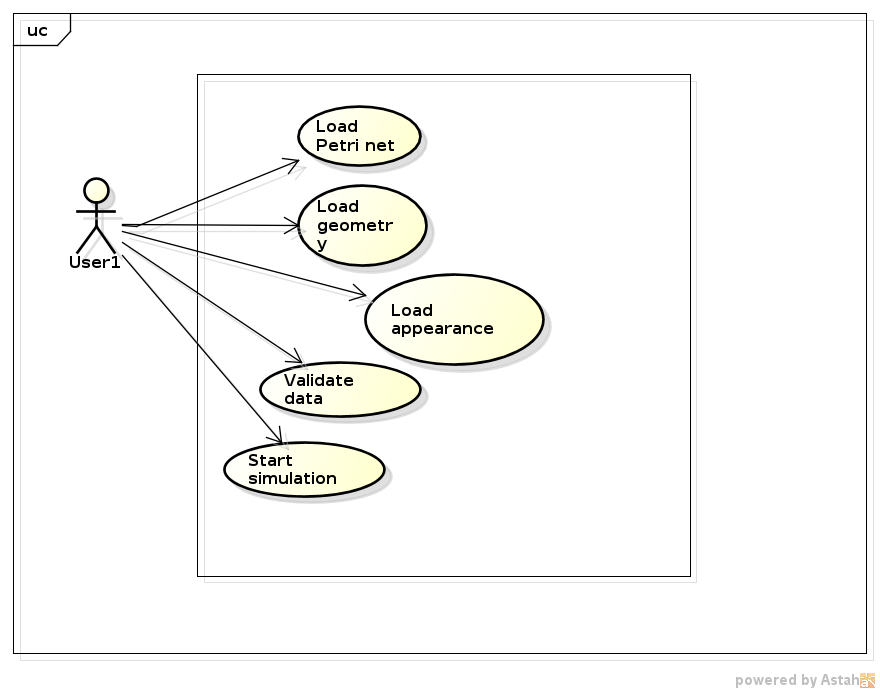
\includegraphics[width=0.5\textwidth]{image/uc-configuration.png}
  \caption{Use cases for the Configuration Editor}
  \label{fig:use-cases-configuration}
\end{center}
\end{figure}